\documentclass{ligodoc}

\usepackage{graphicx}
\usepackage{amssymb}
\usepackage{amsmath}
\usepackage{longtable}
%\usepackage{rotating}
\usepackage[usenames,dvipsnames]{color}
%\usepackage{fancyhdr}
% Some PDFtex-specific options
\usepackage{hyperref}
\usepackage{subfigure}
\usepackage{bm}   %bold math
\usepackage{textcomp}     %non-italic mu
\newcommand{\micro}{\textmu{}}


\ligodccnumber{x}{xx}{xxxx}{xx}{x}
\ligodistribution{LIGO Scientific Collaboration}
\ligodraft

\title{GEO Squeezing Noise Budget}
\author{Kate Dooley, Hartmut Grote, Henning Vahlbruch (\emph{alphabetical order for now})}
\date{Feb. 28, 2012}
\begin{document}

\section{Introduction}
....


\section{Overview of squeezing setup}



\section{OMC parameters}
Table~\ref{tab:OMCparams} summarizes the OMC design parameters.

\begin{table}
\centering
\caption{OMC parameters. Many numbers come from p.12 of the GEO-HF logbook.}
\begin{tabular}{l l l l} %r@{}l r@{}l
\hline
quantity & symbol & value & units \\
\hline
Finesse & F & 160 & \\
round trip length & L & 0.658 & m \\
g-factor & g & 0.735 & \\
waist size & $\omega_0$ & 450 & \micro m \\
free spectral range & FSR & 455.6 & MHz \\
%Michelson sideband frequency & $f_{\mathrm{MI}}$ & 14.90 & MHz \\
%SRC sideband frequency & $f_{\mathrm{SR}}$ & 9.18 & MHz \\
Michelson sideband power transmission & $T_{\mathrm{MI}}$ & 1.01 & $\%$ \\
SRC sideband power transmission & $T_{\mathrm{SR}}$ & 2.71 & $\%$ \\
\hline
\end{tabular}
\label{tab:OMCparams}
\end{table}



\section{Optical losses}
Table~\ref{tab:losses} summarizes our optical loss budget for the
squeezer path.

\begin{table}
\centering
\caption{Optical losses of squeezed beam.}
\begin{tabular}{l l l} %r@{}l r@{}l
\hline
component & power loss & notes \\
\hline
squeezer path Faraday & 3.3\% & \\
output port Faraday & 3.3\% & guess, experienced twice \\
BDO1 transmission & 1\% & experienced twice \\
MSR transmission (when locked) & 1\% & above 1~kHz \\
OMC mode-matching loss & 6\% & \\
OMC AR coating loss & 1\% & \\
OMC internal losses & 14\% & deduced from other measurements \\ 
OMC trans PD detection loss & 9\% & \\
\hline
TOTAL & 63.9\% & multiplied in series \\
\hline
\end{tabular}
\label{tab:losses}
\end{table}


\begin{figure}
\begin{centering}
\includegraphics[width=\textwidth]{/home/kadool/figures/SQZpowerbudget.pdf}
\caption{Optical losses.}
\label{fig:powerbudget}
\end{centering}
\end{figure}



\section{Phase noise from RF sidebands}
The presence of both the carrier contrast defect and the RF sidebands
in the OMC transmitted light results in jitter of the squeezing
quadrature. Figure~\ref{fig:AMPM} provides a pictorial view of the
role of the sidebands in modulating light at the output port. 

\begin{figure}
\begin{centering}
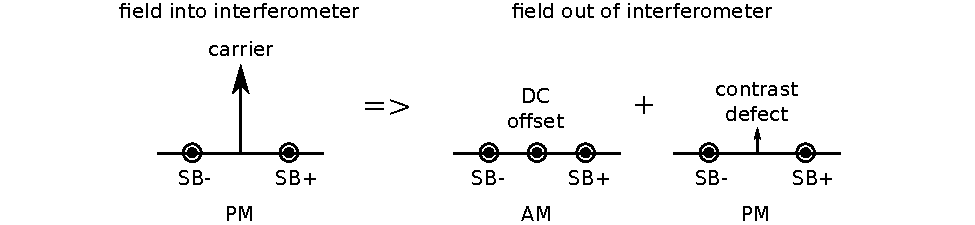
\includegraphics{/home/kadool/figures/AMPM.pdf}
\caption{The RF sidebands (SB+ and SB-) are generated via phase
  modulation of the carrier field. The Michelson interferometer
  rotates the differential carrier field (CR) by 90 deg, but leaves
  all other fields the same, including the RF sidebands and the
  contrast defect (CD). The result is that at the output port, the RF
  sidebands are amplitude modulation (AM) on the carrier, yet continue
  to be phase modulation (PM) on the contrast defect.}
\label{fig:AMPM}
\end{centering}
\end{figure}

Rewriting Eq. 90 from T0900325, the rms fluctuation of the squeezing
quadrature angle, $\Gamma_{\mathrm{rms}}$, is dependent on the ratio
of carrier light with signal, $P_{\mathrm{CR}}$, to light without
signal that is transmitted through the OMC. Examples are the contrast
defect carrier, $P_{\mathrm{CD}}$, and the sidebands, $P_{\mathrm{SB}}$:
\begin{equation}
\Gamma_{\mathrm{rms}} = \sqrt{\frac{P_{\mathrm{SB}}}{P_{\mathrm{CR}}} \left( \frac{1}{\eta} + \epsilon^2 \frac{1-\eta}{\eta} \right)}
\label{eq:Gammarms}
\end{equation}
All powers in this equation are for those transmitted through the OMC,
and the variables $\eta$ and $\epsilon$ are defined as follows:
\begin{equation}
\eta = \frac{P_{\mathrm{CR}}}{P_{\mathrm{CD}}}
\end{equation}
\begin{equation}
\epsilon = \frac{1}{2}\frac{P_{\mathrm{SB+}}-P_{\mathrm{SB-}}}{P_{\mathrm{SB+}}+P_{\mathrm{SB-}}}
\end{equation}
The sideband imbalance is quantified by $\epsilon$ and a sample
measurement of the imbalance (from several years ago) is shown in
Figure~\ref{fig:Hildscan}. Currently, $\epsilon=0.15$. The contrast
defect, commonly quoted as $1/\eta$, can be measured by comparing the
power transmitted through the OMC with and without the dark fringe
offset. The contrast defect is approximately 5\%.

\begin{figure}
\begin{centering}
\includegraphics[width=0.6\textwidth]{Hild_OMCscan.png}
\caption{Snapshot of a scan of the output port by Stefan Hild showing
  the sideband imbalance. In this particular plot, $\epsilon=0.23$. It
  was more recently measured to be $\epsilon = 0.15$.}
\label{fig:Hildscan}
\end{centering}
\end{figure}

Figure~\ref{fig:phirms} shows the dependence of phase noise on
contrast defect for our current sideband imbalance. We expect an rms
phase noise of about $2^\circ$.

\begin{figure}
\begin{centering}
\includegraphics[width=1.1\textwidth]{/home/kadool/GEOHF/projects/SQZphase/rmsphase.pdf}
\caption{RMS phase noise as a function of the ratio of carrier to
  contrast defect in the OMC transmitted beam. The typical operating
  point for GEO is $P_{\mathrm{CR}}/P_{\mathrm{CD}}=20$, which
  corresponds to an RMS phase noise of $1.8^\circ$.}
\label{fig:phirms}
\end{centering}
\end{figure}



\subsection{Manipulating $\Gamma_{\mathrm{rms}}$}
We changed the rms phase noise up to a factor of 4 by reducing the
sideband amplitude and increasing the dark fringe offset. The result
is an improvement in observed squeezing of 1.9~dB to 2.8~dB.




\subsection{Squeezer phase error point}
Our current setup for creating a squeezer to GEO output relative phase
error signal uses the beat of the squeezer sidebands with the
Michelson sidebands in reflection of the OMC which are at 15.2~MHz and
14.9~MHz, respectively. A sample error point spectra is shown in
Figure~\ref{fig:sqzEP} and demonstrates that we measure only 5 mrad
rms phase noise. Our sensor is not measuring the 35~mrad ($\approx
2^\circ$) predicted by the RF sideband model of Eq.~\ref{eq:Gammarms}.

\begin{figure}
\begin{centering}
\includegraphics[width=1.1\textwidth]{/home/kadool/GEOHF/2012/02/16/sqzEP.pdf}
\caption{Calibrated squeezer error point (blue curve), measured as the
  beat between the squeezer sidebands and the RF Michelson sidebands
  in reflection of the OMC. We are limited by dark noise (black curve)
  above 40~kHz.}
\label{fig:sqzEP}
\end{centering}
\end{figure}



\subsection{Contrast defect}
We implement a slow servo called the \emph{noiselock loop} that serves
to change the squeezing quadrature in order to maximize the strain
sensitivity. The need for such a servo arises from the existence of
contrast defect carrier in the OMC transmitted beam. As long as the
amplitude of the contrast defect remains constant in time, so does the
squeezing angle. However, when the amount of contrast defect changes,
so does the angle of the quadrature that produces the best squeezing.


\section{Higher order modes}
We test the effect of higher order modes on the squeezing quadrature
jitter by placing an aperture in the beam path after the OMC. 



\section{Ideas for improvements}

\begin{enumerate}
\item 2nd OMC
\item 

\end{enumerate}



\section{Acknowledgements}


\end{document}



